\documentclass[conference]{IEEEtran}
\IEEEoverridecommandlockouts

% Packages
\usepackage{cite}
\usepackage{amsmath,amssymb,amsfonts}
\usepackage{graphicx}
\usepackage{textcomp}
\usepackage{xcolor}
\usepackage{booktabs}
\usepackage{multirow}
\usepackage{url}
\usepackage{hyperref}
\usepackage{tabularx}
\usepackage{algorithm}
\usepackage{algpseudocode}
\usepackage{listings}
\usepackage{caption}
\usepackage{microtype}
\usepackage{tikz}
\usepackage{subcaption}
\usepackage{amsmath}
\usetikzlibrary{positioning, arrows.meta, shapes.geometric}

\def\BibTeX{{\rm B\kern-.05em{\sc i\kern-.025em b}\kern-.08em
		T\kern-.1667em\lower.7ex\hbox{E}\kern-.125emX}}

\begin{document}
	
	\title{ExRay: Hybrid Interpretable Machine Learning for Malicious Chrome Extension Detection}
	
	\author{\IEEEauthorblockN{Elijah Segura}
		\IEEEauthorblockA{\textit{Department of Computer Science} \\
			\textit{Central Michigan University}\\
			Mount Pleasant, MI, USA \\
			segur1em@cmich.edu}
	}
	
	\maketitle
	
	\begin{abstract}
		Browser extensions present significant security risks, since they operate with elevated privileges and access to sensitive user data. Traditional rule-based detection systems suffer from high false positive rates (61\% as tested. Machine learning approaches, though more accurate, typically function as black boxes that cannot explain their decisions to users. We present ExRay - a hybrid interpretable malware detection system for Chrome extensions, combining static rule-based analysis with an interpretable Random Forest classifier. Our key contribution is semantic aggregation of SHAP (SHapley Additive exPlanations) values into seven domain specific risk categories, helping to increase understanding of classifications. We curated a real-world dataset of 142 Chrome extensions (72 malicious, 70 benign) with labeling from Chrome Web Store removal flags. Our system achieves 82\% cross-validation accuracy and 77\% hold-out test accuracy, a 20 percentage point improvement over the rule-based approach, while reducing false positive rates by 35 percentage points. The interactive web interface enables users to explore a detailed analysis on why an uploaded or preset extension is classified as malicious or benign, and comparison between the two approaches.
	\end{abstract}
	
	
	\section{Introduction}
	Browser extensions have become ubiquitous tools for enhancing web browsing functionality. As of 2024, the Chrome Web Store hosted over 180,000 extensions with billions of cumulative downloads. However, this popularity has made extensions an attractive attack vector for malicious actors \cite{287202}. Malicious extensions can steal credentials, inject advertisements, track user behavior, and exfiltrate sensitive data. All while appearing as legitimate productivity tools.
	
	\subsection{Problem Statement}
	The detection of malicious browser extensions presents a challenging security problem that traditional approaches fail to adequately address.
	
	\textbf{Rule-Based Systems}: Traditional signature and heuristic-based detection methods suffer from high false positive rates. In our experiments, our rule-based analysis incorrectly flagged 61\% of benign as extensions as potentially malicious, insufficient for user trust and reliability. These type of systems struggle to distinguish between legitimate uses of APIs (e.g. password managers requiring credential access) and malicious abuse of the same capabilities. 
	
	\textbf{Black-Box Machine Learning}: While ML-based approaches achieve higher accuracy, they typically operate as opaque classifiers that provide probability scores without explanation \cite{unknown}. If a security analyst cannot understand why an extension was flagged, it introduces difficultly for verifying decisions, prioritizing responses, or improving detection rules. This lack of interpretability is particularly problematic in security contexts where professionals must justify blocking decisions \textbackslash{}cite\{baghirov\_2024\}.
	
	\textbf{The Interpretability Gap}: A fundamental tensions exists between detection accuracy and explainability. Deep learning approaches such as neural networks for JavaScript analysis \cite{9020870} achieve strong performance but sacrifice interpretability. Conversely, simple rule-based systems are transparent but miss sophisticated threats.
	
	\subsection{Our Contribution}
	We address this gap with a hybrid interpretable malware detection system that provides both accurate classification and human-understandable explanations. Our primary contribution is \textbf{semantic aggregation of SHAP values}, which transforms raw feature importances into meaningful risk categories that security practitioners can understand and act upon.
	
	By transforming raw features importance into meaningful risk categories, users can understand and act upon predictions presented by the system.
	
	Instead of presenting feature names like:
	\begin{itemize}
		\item \texttt{perm\_scripting}: 0.15
		\item \texttt{tfidf\_eval}: 0.12
		\item \texttt{perm\_webRequest}: 0.08
	\end{itemize}
	
	Our system aggregates these into interpretable categories:
	\begin{itemize}
		\item \textbf{Permissions Risk (26\% impact)}: scripting, webRequest, cookies
		\item \textbf{Code Behavior (18\% impact)}: eval usage, dynamic function creation
		\item \textbf{Network Activity (11\% impact)}: fetch calls, XMLHttpRequest
	\end{itemize}
	
	We can summarize our work with 5 major contributions:
	
	\begin{enumerate}
		\item A \textbf{hybrid analysis architecture} combining separate transparent rule-based scoring with accurate ML classification
		\item \textbf{SHAP-based category aggregation} that groups feature importance's into seven semantic risk categories
		\item A \textbf{curated dataset} of 142 Chrome extensions with ground-truth malware labels
		\item An \textbf{interactive web interface} enabling exploration of risk factors with detailed explanations
		\item \textbf{Comprehensive evaluation} demonstrating 20+ percentage point accuracy improvement over rule-based systems
	\end{enumerate}
	
	\section{Related Work}
	
	\subsection{Browser Extension Security}
	
	Sanchez-Rola et al.\ \cite{203846} conducted one of the first comprehensive security analyses of browser extension resource control policies, identifying vulnerabilities in how extensions manage access to web content. Their work highlighted the inadequacy of permission-based security models, motivating our multi-factor approach that examines both manifest permissions and actual code behavior.
	
	Kim and Lee \cite{287202} demonstrated that browser extensions can be exploited for privilege escalation attacks, with malicious extensions leveraging legitimate API access to compromise browser security. Their findings emphasizes the importance of detecting not just obviously malicious patterns, but also subtle capability combinations that enable attacks. Our permission-risk scoring incorporates insights from their attack taxonomy.
	
	Laperdrix et al.\ \cite{272161} showed that browser extensions can be fingerprinted through their injected style sheets, enabling tracking across sessions. While their work focuses on privacy implications, it demonstrates the extensive capabilities available to extensions, those that malicious actors can abuse.
	
	\subsection{Machine Learning for Malware Detection}
	
	The application of machine learning to malware detection has received extensive attention. Gaber et al.\ \cite{article} provide a systematic literature review covering 290 studies, identifying feature extraction, model selection, and evaluation methodology as critical success factors. Our work focuses on their identified gap in interpretability by incorporating SHAP-based explanations.
	
	Stokes et al.\ \cite{9020870} developed ScriptNet, a neural network approach for malicious JavaScript detection using LSTMs. While their model achieves strong performance, it operates as a black box. Our Random Forest approach sacrifices some potential accuracy for interpretability, enabling security analysts to understand and verify classification decisions.
	
	Gobbi and Kinder \cite{10734052} presented GENIE for detecting malicious npm packages using semantic analysis. Their work on the JavaScript ecosystem  is similar to ours, though we focus specifically on browser extensions with their unique manifest-based permission model. Both approaches recognize the importance of understanding code behavior beyond simple pattern matching.
	
	\subsection{Explainable AI for Security}
	
	The need for interpretable ML in security contexts has been well established. Lin and Chang \cite{unknown} surveyed interpretation methods for ML-based malware detection, categorizing approaches by explanation granularity and identifying SHAP as particularly suitable for feature-based models. Our category aggregation extends their framework by grouping SHAP values into domain-specific risk categories.
	
	To et al.\ \cite{10288922} developed MalDEX, an explainable malware detection system using ensemble learning with SHAP visualizations. Our work differs by focusing on browser extensions rather than executables, and by introducing semantic category aggregation that produces more actionable explanations.
	
	Baghirov \cite{baghirov_2024} examined advanced ML and interpretability for Windows malware detection, emphasizing the importance of human-understandable explanations for security operations. Our approach extends these insights to the browser extension domain, where the permission model provides natural semantic categories for explanation.
	
	\subsection{Hybrid Detection Approaches}
	
	Hybrid systems combining rules and ML have shown promise across security domains. Zeeshan and Amjad \cite{10606032} demonstrated effective hybrid malware classification for PDFs, achieving improved accuracy over single-method approaches. Our architecture similarly leverages the complementary strengths of rule-based transparency and ML accuracy, using rules for detailed threat scoring, while ML provides overall classification.
	
	
	\section{Methodology and System Design}
	
	\subsection{System Architecture}
	Our system follows a pipeline architecture as shown in Figure \ref{fig:architecture}. User-uploaded extensions pass through feature extraction, dual analysis (rules + ML), and explainability modules before results are displayed in an interactive interface.
	\begin{figure}[htbp]
		\centering
		\resizebox{\columnwidth}{!}{
			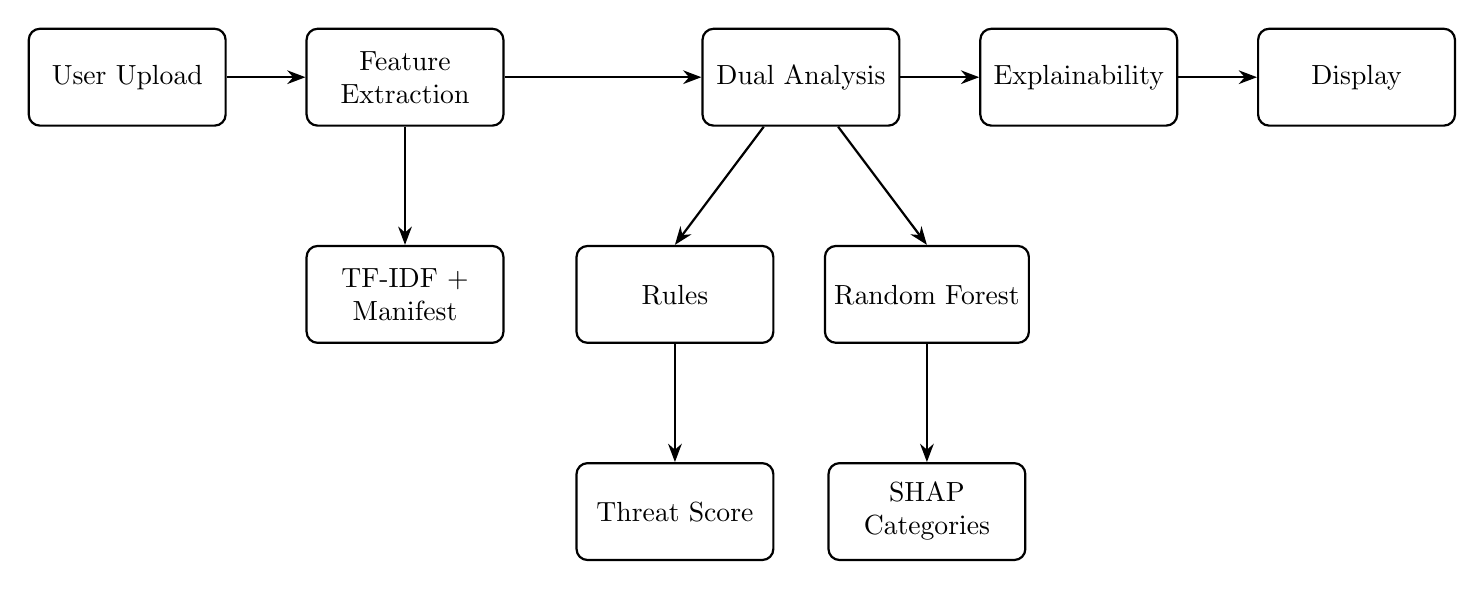
\begin{tikzpicture}[
				% INCREASED horizontal spacing (second number) to 2cm to prevent overlap
				node distance=1.5cm and 2cm, 
				box/.style={
					rectangle, 
					draw, 
					rounded corners, 
					align=center, 
					minimum height=3.5em, 
					minimum width=2.5cm, 
					fill=white,
					thick
				},
				arrow/.style={-Stealth, thick}
				]
				
				% --- 1. Top Row (Main Pipeline) ---
				\node[box] (upload) {User Upload};
				\node[box, right=1cm of upload] (extract) {Feature\\Extraction};
				
				% Explicitly wider gap here to fit the children nodes underneath
				\node[box, right=2.5cm of extract] (dual) {Dual Analysis};
				
				\node[box, right=1cm of dual] (explain) {Explainability};
				\node[box, right=1cm of explain] (display) {Display};
				
				% Connect Main Pipeline
				\draw[arrow] (upload) -- (extract);
				\draw[arrow] (extract) -- (dual);
				\draw[arrow] (dual) -- (explain);
				\draw[arrow] (explain) -- (display);
				
				% --- 2. Second Row (Components) ---
				
				% Under Feature Extraction (TF-IDF)
				\node[box, below=of extract] (tfidf) {TF-IDF +\\Manifest};
				\draw[arrow] (extract) -- (tfidf);
				
				% Under Dual Analysis (Split into two)
				% xshift moves them horizontally relative to the center of 'dual'
				\node[box, below=of dual, xshift=-1.6cm] (rules) {Rules};
				\node[box, below=of dual, xshift=1.6cm] (rf) {Random Forest};
				
				\draw[arrow] (dual) -- (rules.north);
				\draw[arrow] (dual) -- (rf.north);
				
				% --- 3. Third Row (Outputs) ---
				\node[box, below=of rules] (threat) {Threat Score};
				\node[box, below=of rf] (shap) {SHAP\\Categories};
				
				\draw[arrow] (rules) -- (threat);
				\draw[arrow] (rf) -- (shap);
				
			\end{tikzpicture}
		}
		\caption{High-level system architecture showing dual analysis paths}
		\label{fig:architecture}
	\end{figure}
	
	\subsection{Feature Extraction}
	We extract 1,019 features from each extension, combining static code analysis with manifest inspection:
	
	\textbf{TF-IDF Code Features (1,000)}: We apply Term Frequency-Inverse Document Frequency vectorization to all JavaScript files in an extension, using a vocabulary of 1,000 terms. This captures code patterns including API calls, variable names, and suspicious strings associated with malicious behavior.
	
	\textbf{Manifest Permission Features (19)}: Binary features encode the presence of permissions:
	\begin{itemize}
		\item High-risk: \texttt{scripting}, \texttt{webRequest}, \\ \texttt{management}, \texttt{debugger}
		\item Medium-risk: \texttt{tabs}, \texttt{cookies}, \texttt{downloads}, \\ \texttt{nativeMessaging}
		\item Low-risk: \texttt{storage}, \texttt{notifications}, \\ \texttt{contextMenus}
		\item Host access: \texttt{<all\_urls>}, broad host patterns
		\item CSP bypass: \texttt{unsafe-eval} in Content Security Policy
	\end{itemize}
	
	
	\subsection{Rule-Based Threat Scoring}
	
	Our rule engine analyzes extensions using Abstract Syntax Tree (AST) parsing of JavaScript code via the Esprima library. Findings are scored using a weighted saturation system:
	
	
	\begin{equation}
		\text{Score}_{\text{raw}} = \sum_{c \in \text{categories}} \min\left(\sum_{f \in c} w_f, S_c\right)
	\end{equation}
	
	where $w_f$ is the weight for finding $f$ and $S_c$ is the saturation limit for category $c$. Saturation prevents a single category from dominating the score. Table \ref{tab:weights} shows our scoring weights.
	
	\begin{table}[h]
		\centering
		\caption{Threat Scoring Weights by Category}
		\label{tab:weights}
		\begin{tabular}{lcc}
			\toprule
			\textbf{Category} & \textbf{Weight} & \textbf{Saturation} \\
			\midrule
			Obfuscation & 25 & 100 \\
			CSP Bypass & 20 & 40 \\
			Suspicious URL & 20 & 100 \\
			Dangerous DOM & 15 & 60 \\
			Risky API & 15 & 100 \\
			Permissions & 10 & 100 \\
			Data Exfiltration & 10 & 50 \\
			\bottomrule
		\end{tabular}
	\end{table}
	
	To prevent large extensions from being unfairly penalized, we apply logarithmic size normalization:
	
	\begin{equation}
		\text{Score}_{\text{norm}} = \text{Score}_{\text{raw}} \times \frac{1}{\log_{10}(1 + n_{\text{files}})}
	\end{equation}
	
	\subsection{Machine Learning Classification}
	We train a Random Forest classifier with 100 trees using class-balanced weights to handle dataset imbalance. The model predicts malicious probability $P(y=1|x)$ for feature vector $x$.
	
	\textbf{Model Configuration}:
	\begin{itemize}
		\item Algorithm: Random Forest (scikit-learn)
		\item Trees: 100 estimators
		\item Class weights: Balanced
		\item Features: 1,019 (TF-IDF + manifest)
	\end{itemize}
	
	
	\subsection{SHAP-Based Category Aggregation}
	
	One key innovation is semantic aggregation of SHAP values. We use TreeExplainer with 50 background samples to compute feature contributions, then aggregate into seven risk categories based on domain knowledge: \ref{alg:alg1}
	
\begin{algorithm}[h]
	\caption{SHAP Category Aggregation}
	\label{alg:alg1}
	\begin{algorithmic}[1]
		\Require Feature vector $x$, SHAP values $\phi$, feature names $F$
		\Ensure Categorized risk factors $R$
		\State $C \gets \{\text{Permissions, Security, Behavior, Network,}$
		\Statex \hskip2em $\text{DOM, Storage, Patterns}\}$
		\For{\textbf{each} category $c \in C$}
		\State $R[c] \gets \{\text{impact}: 0, \text{features}: []\}$
		\EndFor
		\For{\textbf{each} feature $i$ with $\phi_i \neq 0$}
		\State $c \gets \textsc{GetCategory}(F[i])$
		\State $R[c].\text{impact} \gets R[c].\text{impact} + |\phi_i|$ \Comment{Sum absolute impact}
		\State $R[c].\text{features}.\text{append}(\{\text{name}: F[i], \text{imp}: \phi_i\})$
		\EndFor
		\State \Return $R$ sorted by impact
	\end{algorithmic}
\end{algorithm}


The \texttt{GetCategory} function maps features to categories using pattern matching:
\begin{itemize}
	\item \texttt{perm\_*} $\rightarrow$ Permissions
	\item \texttt{unsafe\_eval} $\rightarrow$ Security
	\item \texttt{eval}, \texttt{innerHTML} $\rightarrow$ Behavior
	\item \texttt{http*}, \texttt{url*} $\rightarrow$ Network
	\item \texttt{document.*} $\rightarrow$ DOM
	\item \texttt{storage}, \texttt{cookie} $\rightarrow$ Storage
	\item Other TF-IDF terms $\rightarrow$ Code Patterns
\end{itemize}


\subsection{Confidence-Based Filtering}
To reduce false positives, we implement confidence scoring that considers the context:

\begin{equation}
	\text{Confidence} = C_{\text{base}} \times M_{\text{path}} \times M_{\text{safety}}
\end{equation}

where $C_{\text{base}}$ is the base confidence for the finding type, $M_{\text{path}}$ reduces confidence for test/vendor files, and $M_{\text{safety}}$ reduces confidence when safety indicators (try/catch, sanitization) are present.

Findings are filtered by severity-specific thresholds:
\begin{itemize}
	\item Critical: 0.4 (keeps most findings)
	\item High: 0.5
	\item Medium: 0.6
	\item Low: 0.7 (higher bar for minor findings)
\end{itemize}


\subsection{Interactive Web Interface}

We provide a Flask-based web interface enabling:
\begin{itemize}
	\item Extension upload via ZIP file or preset selection \ref{fig:first-screen}
	\item Visual threat score scale with severity coloring \ref{fig:second-screen}
	\item Expandable risk category exploration \ref{fig:risk-factors}
	\item Analysis breakdown and full JSON export \ref{fig:analysis-info}
	\item Detailed threat score breakdown and analysis \ref{fig:breakdown}
	\item Per-finding confidence scores and descriptions with specific locations \ref{fig:risk-summary}
	\item Detailed findings with specific code snippets \ref{fig:detailed-findings}

\end{itemize}

\begin{figure}[htbp]
	\centering
	% Row 1
	\begin{subfigure}{0.45\textwidth}
		\includegraphics[width=\linewidth]{figures/first-screen}
		\caption{Extension upload}
		\label{fig:first-screen}
	\end{subfigure}
	\hfill
	\begin{subfigure}{0.45\textwidth}
		\includegraphics[width=\linewidth]{figures/second-screen}
		\caption{Threat score scale}
		\label{fig:second-screen}
	\end{subfigure}
	
	\medskip
	
	% Row 2
	\begin{subfigure}{0.45\textwidth}
		\includegraphics[width=\linewidth]{figures/risk-factors}
		\caption{Risk categories}
		\label{fig:risk-factors}
	\end{subfigure}
	\hfill
	\begin{subfigure}{0.45\textwidth}
		\includegraphics[width=\linewidth]{figures/analysis-info}
		\caption{Analysis breakdown}
		\label{fig:analysis-info}
	\end{subfigure}
	
	\caption{Interface Overview (Part 1): Initial upload and high-level risk assessment.}
	\label{fig:interface-part1}
\end{figure}

\begin{figure}[htbp]
	\centering
	% Row 3
	\begin{subfigure}{0.45\textwidth}
		\includegraphics[width=\linewidth]{figures/breakdown}
		\caption{Detailed threat breakdown}
		\label{fig:breakdown}
	\end{subfigure}
	\hfill
	\begin{subfigure}{0.45\textwidth}
		\includegraphics[width=\linewidth]{figures/risk-summary}
		\caption{Confidence scores}
		\label{fig:risk-summary}
	\end{subfigure}
	
	\medskip % Space between rows
	
	% Row 4
	\begin{subfigure}{0.45\textwidth} 
		\centering
		\includegraphics[width=\linewidth]{figures/detailed-findings}
		\caption{Specific findings with code}
		\label{fig:detailed-findings}
	\end{subfigure}
	
	\caption{Interface Overview (Part 2): Detailed scoring and code-level findings.}
	\label{fig:interface-part2}
\end{figure}


\section{Evaluation}

\subsection{Dataset}

We curated a dataset of 142 Chrome extensions with ground-truth labels:

{\sloppy
	\textbf{Malicious Extensions (72)}: Collected via Chrome-Stats API with criteria \texttt{obsolete=Exists} and \texttt{obsoleteReason=``malware''}. These extensions were flagged and removed by Google for malicious behavior, providing reliable labels.
	
	\textbf{Benign Extensions (70)}: Collected with criteria \texttt{obsolete=NotExists} and \texttt{isTrustedPublisher=Exists}. Active extensions from verified publishers represent legitimate software.
}

Table \ref{tab:dataset} summarizes the dataset statistics.

\begin{table}[h]
	\centering
	\caption{Dataset Statistics}
	\label{tab:dataset}
	\begin{tabular}{lcc}
		\toprule
		\textbf{Metric} & \textbf{Benign} & \textbf{Malicious} \\
		\midrule
		Extensions & 70 & 72 \\
		Total Files & 15,752 & 4,203 \\
		Avg JS Files/Ext & 225 & 58 \\
		\bottomrule
	\end{tabular}
\end{table}

	

\subsection{Evaluation Methodology}

We employ two complementary evaluation approaches:

\textbf{5-Fold Stratified Cross-Validation}: Provides honest performance estimates with variance measurement across the full dataset.

\textbf{70/30 Train-Test Split}: Simulates real-world deployment where the model is trained on historical data and tested on unseen extensions.

\subsection{Cross-Validation Results}

Table \ref{tab:cv} presents 5-fold cross-validation results.

\begin{table}[h]
	\centering
	\caption{5-Fold Cross-Validation Results (n=142)}
	\label{tab:cv}
	\begin{tabular}{lcc}
		\toprule
		\textbf{Metric} & \textbf{Mean} & \textbf{Std Dev ($\pm$2$\sigma$)} \\
		\midrule
		Accuracy & 82.36\% & 12.57\% \\
		Precision & 82.24\% & 13.10\% \\
		Recall & 83.33\% & 13.68\% \\
		F1-Score & 82.70\% & 12.43\% \\
		\bottomrule
	\end{tabular}
\end{table}

Per-fold accuracy: [93.10\%, 75.86\%, 78.57\%, 85.71\%, 78.57\%]. The variance reflects the challenge of small-dataset evaluation, which motivated our reporting of confidence percentages.

\subsection{Hold-Out Test Results}

Table \ref{tab:holdout} shows performance on the 30\% held-out test set (43 extensions).

\begin{table}[h]
	\centering
	\caption{Hold-Out Test Results (43)}
	\label{tab:holdout}
	\begin{tabular}{lc}
		\toprule
		\textbf{Metric} & \textbf{Score} \\
		\midrule
		Accuracy & 76.74\% \\
		Precision & 75.00\% \\
		Recall & 81.82\% \\
		F1-Score & 78.26\% \\
		False Positive Rate & 28.57\% \\
		False Negative Rate & 18.18\% \\
		\bottomrule
	\end{tabular}
\end{table}

The confusion matrix shows 15 true negatives, 18 true positives, 6 false positives, and 4 false negatives. The model prioritizes recall (identifying malicious extensions) over precision, which is more appropriate for a security screening tool.

\subsection{Comparison with Rule-Based System}

Table \ref{tab:comparison} compares our ML approach against the rule-based baseline.

\begin{table}[h]
	\centering
	\small
	\caption{ML vs Rule-Based Comparison}
	\label{tab:comparison}
	\begin{tabular}{lccc}
		\toprule
		\textbf{Metric} & \textbf{Rules} & \textbf{ML} & \textbf{Improvement} \\
		\midrule
		Accuracy & 57.43\% & 76.74\% & +19.3 pp \\
		Precision & 56.52\% & 75.00\% & +18.5 pp \\
		Recall & 75.00\% & 81.82\% & +6.8 pp \\
		FPR & 61.22\% & 28.57\% & -32.7 pp \\
		\bottomrule
	\end{tabular}
\end{table}

The most significant improvement is in false positive rate reduction. Rules flagged 61\% of benign extensions, which is impractical. Our ML approach reduces this to 29\%.

\subsection{Interpretability Assessment}

Our category aggregation produces explanations that map directly to security concepts:

\subsubsection*{Example Output for Malicious Extension}
\begin{description}
	\item[Permissions (32\% impact)] \hfill \\
	\textbullet\ \texttt{scripting}: Execute arbitrary JS \\
	\textbullet\ \texttt{webRequest}: Intercept traffic
	
	\item[Behavior (28\% impact)] \hfill \\
	\textbullet\ \texttt{eval}: Dynamic code execution \\
	\textbullet\ \texttt{atob}: Base64 decoding (obfuscation)
	
	\item[Network (15\% impact)] \hfill \\
	\textbullet\ \texttt{fetch}: External communication
\end{description}

This format allows users to quickly understand the specific risk factors that contribute to classification.

\subsection{Limitations}

\textbf{Overfitting}: We observed a 23 percentage point gap between training accuracy (100\%) and test accuracy (77\%), indicating some overfitting. With 1,019 features and 142 samples, our feature-to-sample ratio exceeds typical recommendations.

\textbf{Dataset Size}: Our dataset of 142 extensions, while carefully curated, limits generalization. Cross-validation variance of $\pm$12\% reflects this limitation.

\textbf{Temporal Bias}: Malicious extensions in our dataset are historical (already removed), potentially not representing emerging attack techniques.

% ============================================
% CONCLUSION
% ============================================
\section{Conclusion}

We presented a hybrid interpretable malware detection system for Chrome extensions that bridges the gap between detection accuracy and explainability. By aggregating SHAP values into semantic risk categories, we enable users or security practitioners to understand classification decisions without sacrificing the accuracy benefits of machine learning.

Our system achieves 77-82\% accuracy, representing a 20+ percentage point improvement over rule-based approaches while reducing false positive rates by over 30 percentage points. The interactive interface contributes to usability, in-depth analysis, and comparison between the ML and rule-based approaches.

Future work includes expanding the dataset to 200+ extensions, implementing deep learning approaches with attention-based explanations, and conducting user studies to evaluate explanation quality.

% ============================================
% REFERENCES
% ============================================
\bibliographystyle{IEEEtran}
\bibliography{references}

\end{document}
